
\documentclass{article}
\usepackage{geometry}
\usepackage{float}
\usepackage{graphicx}
\usepackage{caption}
\usepackage{multirow}
\usepackage{array}
\usepackage[affil-it]{authblk}
\usepackage{lscape}
\usepackage[bottom]{footmisc}
\usepackage{amssymb}
\usepackage{amsmath}
\usepackage{color,hyperref}

\geometry{top=1in, bottom=1in}
\setlength{\parindent}{0pt}
\setlength{\parskip}{12pt}

\definecolor{CarolinaBlue}{RGB}{75, 156, 211}
\hypersetup{colorlinks,breaklinks,linkcolor=CarolinaBlue,urlcolor=CarolinaBlue,anchorcolor=CarolinaBlue,citecolor=black}

\title{ECON 390: Final Project}
\author{Alex Marsh}
\date{Due: December 9, 2021}

\begin{document}

\maketitle

\section*{Directions and Context}

In the US, anyone who needs treatment for kidney dialysis to treat End Stage Renal Disease (ESRD) automatically qualifies for Medicare regardless of their age. As such, there is lots of data about dialysis clinics and their operations collected by government agencies, specifically CMS. While these cost reports could be a gold mine for any sort of economic modeling we would like to do with dialysis clinics, these cost reports are very dirty, to say the least. This will be a chance for you to work with real world data to see many of the issues you will encounter when working with real data.

	To get started and to learn a little bit about the industry, I recommend reading the \href{https://academic.oup.com/qje/article-abstract/135/1/221/5607794?redirectedFrom=fulltext}{following paper}: ``How Acquisitions Affect Firm Behavior and Performance: Evidence from the Dialysis Industry" by Eliason, Heebsh, McDevitt, and Roberts. You do not need to read section 5, but it is interesting. The paper is not too technical and it's a very good paper.\footnote{I also heard the RAs on this project were really smart, and one of them is a really good instructor.} Also, you should listen to this episode of the \href{https://freakonomics.com/podcast/dialysis/}{Freakonomics podcast} up to the 25 minute mark or the first commercial break during the episode. The paper and podcast will give you the relevant industry background to understand the data.
	
	\textbf{What you should submit}: Submit both the pdf and the RMarkdown file just like for the problem sets. For questions 1 and 2, unless a question is asked that requires words to answer, you do not need to write anything. However, for question 3, I am hoping for writing and analysis. \textit{\textbf{Do not just give me code, plots, and tables}}. Remember that you can write text in RMarkdown documents outside the R code chunks. If you're unsure how to do this, please ask me.

\section*{Question 1: Download Data}

I want you to download the data from the NBER website. There are three types of files: report files (abbreviated rpt), numeric (nmrc), and alphabetical (alpha) data. The years we will be looking at are years 1998 to 2010. For 2010, the links to download each type of data can be seen below:
\begin{itemize}
	\item rpt: \href{http://www.nber.org/hcris/265-94/rnl_rpt265_94_2010.csv}{\tt\bf http://www.nber.org/hcris/265-94/rnl\_rpt265\_94\_2010.csv}
	\item nmrc: \href{http://www.nber.org/hcris/265-94/rnl_nmrc265_94_2010_long.csv}{\tt\bf http://www.nber.org/hcris/265-94/rnl\_nmrc265\_94\_2010\_long.csv}
	\item alpha: \href{http://www.nber.org/hcris/265-94/rnl_alpha265_94_2010_long.csv}{\tt\bf http://www.nber.org/hcris/265-94/rnl\_alpha265\_94\_2010\_long.csv}
\end{itemize}
So to get the data for other years, the only thing that needs to change is the 2010 in the link.

\textbf{Your job}: Download all the cost report data from 1998 to 2010 by looping over the years and types of data (i.e. rpt, nmrc, alpha). To be clear, \textit{\textbf{you should be using R to download the data}}.

Some notes: 
\begin{enumerate}
	\item You should create a directory for the entire final project,
	\item You should be saving these files that are downloaded in a directory within the final project directory titled ``hcris\_raw".
	\item Note that both the alpha and nmrc files include ``\_long" at the end of the url whereas the rpt data does not. Keep this in mind when you're writing your code.
	\item You include a "switch" in the code that indicates whether or not the data should be downloaded. This is to prevent the data from being downloaded every time you run the script. There are other ways to do this, so it doesn't have to be a TRUE/FALSE switch, but regardless, you should implement something that prevents the data from being downloaded every time the entire script is run.
	\item While I mentioned this in class, I will remind you of the download.file() function.
\end{enumerate}

\section*{Question 2: Cleaning The Data}

Now that the data are downloaded to your computer, you must read in the data, extract the relevant variables, merge the data together, and then clean it. This process will be the most complicated and challenging.

Along with the project, I have supplied a .csv file for the variables you should extract. The alpha and nmrc data files are in \textit{long} format. We have discussed this a bit in class. It is worth visiting the alpha and nmrc links above to get a feel for what the data look like. Here is my explanation:

\subsection*{Reformatting The Raw Data}

\begin{itemize}
	\item For each report number (rpt\_rec\_num), the variables wksht\_cd, line\_num, and clmn\_num form a variable. Think of these like an Excel spreedsheet: The worksheet is the worksheet in the Excel document, the line number is the row number and the column number is the column number. Then, the value of whichever item is identified is in the variable itm\_val\_num.
	\item If you're still unclear how the data are structured, view the csv file that I included. Each facility for each year has a report number. The variable that we are interested in is identified via a combination of the worksheet, the line number, and the column number. 
	\item We want to convert this long data into a wide panel. In the resulting wide data, each row will be a report, for a given facility, for that year. The columns will be the variables that we are interested in in the csv file. The resulting data can be seen below: 

	\begin{figure}[H]
		\centering
		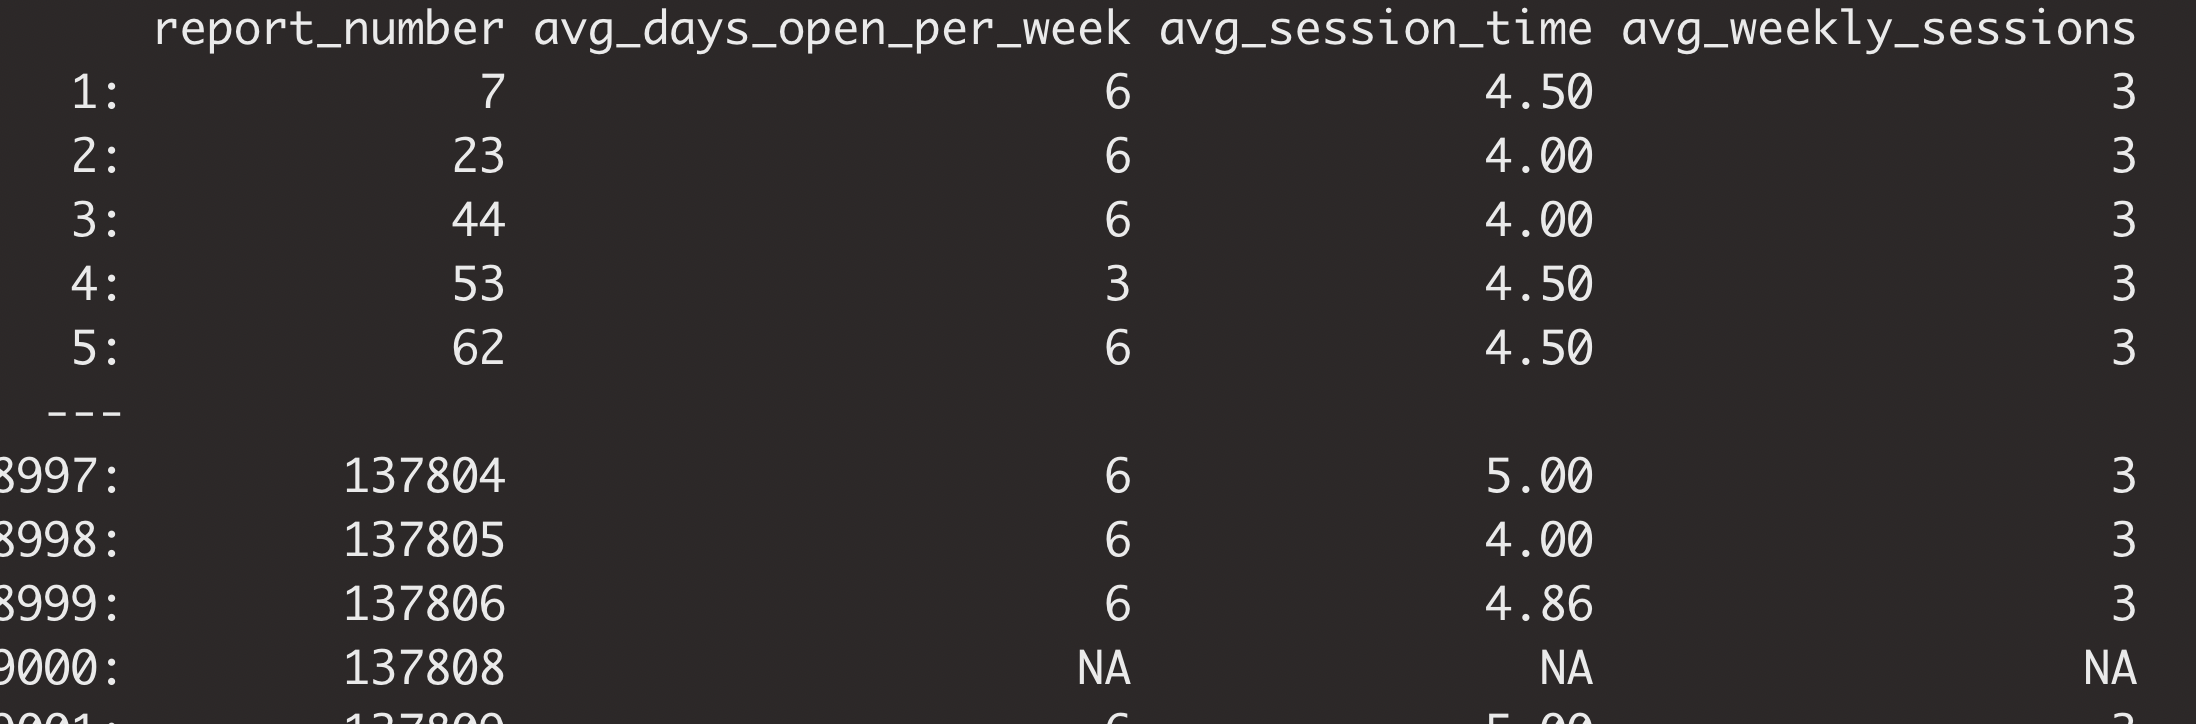
\includegraphics[scale=0.4]{wide_panel}
	\end{figure}
	
	\item Note: You need to create a key from the worksheet, line numbers, and column numbers. The idea is that this key can be how you join it to the alpha and nmrc data and then reshape the data from long to wide. For example, the key for the facility name (the first variable in the csv included with the final project) should be ``S000001001000100" where the worksheet is ``S000001", the line number is ``00100", and the column number is ``0100".
	\item Important: Because the line and column numbers can be accidentally be converted from character data to number data, you have to be very careful with the leading zeros.  \textit{The line number should always have 5 digits and the column number should always have 4 digits}. Before creating the keys, make sure this is the case. For example, if the line number mentioned in the bullet above appears as 100 rather than 00100, you must add two leading zeros. The function str\_pad() in the stringr package should be very useful.
	\item You need to do this process twice for the alpha data and the nmrc data and then join the data together on the report number.
	\item After getting the data in the wide format, you need to merge in two variables from the rpt data. For some reason, some of the report dates are missing in the alpha and nmrc. However, they are present in the rpt data. Therefore, take the resulting data from the bullet point above, and merge that data set with the rpt data for the variables fy\_bgn\_dt and fy\_end\_dt. The variables stand for financial year beginning date and financial year end date.
	\item Add a variable called ``year" that is simply the year of the report.
	\item Finally, save the resulting data as a csv file titled something along the lines as hcris\_YEAR.csv where YEAR is the year of the report. This can be done with the functions write\_csv() if you're tidyverse or fwrite() if you're using data.table. Save these files in a new directory titled hcris\_cleaned that is also in the directory you created for the final project. To be clear, in the final project directory, you should now have two ``subdirectories" titled hcris\_cleaned and hcris\_raw. The data you downloaded should be located in the raw folder, and the data you just reformatted should be located in the cleaned folder. Also, to be clear, in the cleaned folder, you should now have 13 files.
	\end{itemize}
	
	\subsection*{Cleaning The Reformatted Data}
	
	Now that the data are reformatted into the format we will be using, it is time to read all the data in and rbind them. There are variables ways to do it. One way is to read in the 1998 data and call this hcris\_data. Then loop over the years 1999 to 2010, read each year in, call it temp\_data, and then rbind it with hcris\_data. Another way to do it is to use list.files(), lapply(), and then fread() (or read\_csv() in tidyverse). To be clear, hcris\_data should be all the data from 1998 to 2010 that is combined using rbind.
	
	Congratulations, once you've got this far, you've done a lot of challenging work. Be proud of yourself. Now, we need to actually clean the data. Unfortunately, this data set is very messy. This is your first real taste at what real-world data are like. I bet you'll be grateful for my simulated data after all this is over. :)
	
	\begin{enumerate}
		\item First, drop any observations where prvdr\_num is missing. If we were actually cleaning this data, I think there is a way to recover these provider numbers by matching them with the report numbers, but this project is already going to be long enough.
		\item Now, let's start easy. There are some cost data that some clinics reported as negatives. This is bad. As such, replace the original variable with the absolute value of the original variable. Note, you should \textit{not} create a new variable when doing this; you should be replacing the original with the absolute values. These variables include: epo\_cost, epo\_net\_cost, and epo\_rebates.
		\item Next, for epo\_rebates, replace missing values with 0. \textit{Only do this for epo\_rebates right now.}
		\item Next, make sure epo\_cost is a numeric variable. There are lots of missing epo\_cost and epo\_net\_cost observations. We will go through a bunch of cases and make logical inferences on what these values should be. Here's a little context. epo\_cost is the cost of the administered drug Epogen to the clinic. epo\_rebates is the amount of rebates the clinic got from the drug companies. So epo\_net\_cost should equal epo\_cost minus epo\_rebates. The issue is that sometimes missing values mean that the variable was 0 but sometimes they are legitimately missing. We must decide which is which.
		\begin{enumerate}
			\item First look where epo\_cost is missing, epo\_net\_cost is not, and epo\_rebates equals 0. For these observations, set epo\_cost equal to epo\_net\_cost.
			\item Next, look where epo\_cost is missing, epo\_net\_cost is not, and epo\_rebates does not equal 0. Set epo\_cost to epo\_net\_cost plus epo\_rebates.
			\item Next, look where epo\_cost is missing, epo\_net\_cost is also missing, epo\_rebates is 0. Set both epo\_cost \textit{and} epo\_net\_cost to 0. Be careful and make sure to modify both variables at the same time. 
			\item The remaining combination we have is a weird one. Look where epo\_cost is missing, epo\_net\_cost is missing, and epo\_rebates is not zero. This implies epo was used but the costs are missing. There is also a variable called epo\_total which is the total amount of epo used during the financial year. I would leave these as legitimately missing as we don't really know what to do with them.
			\item Next, take observations where epo\_cost is not missing and epo\_net\_cost is missing. Replace epo\_net\_cost with epo\_cost minus epo\_rebates. Now if you look at the observations where epo\_cost is missing or epo\_net\_cost is missing, it is only the 33 observations that we didn't know what to do with.
		\end{enumerate}
		\item Next, there are some observations where epo\_cost is less than epo\_net\_cost. This should not be able to happen. For these observations, switch epo\_cost with epo\_net\_cost and epo\_net\_cost with epo\_cost. It is important to do this all at one time.
		\item Congrats, the epo variables are cleaned (except, not really...). The next thing you need to do is fix one incorrect provider number. I came across this while working on these reports. Take the observations where prvdr\_num equals ``322664" (this should be exactly one observations) and change the prvdr\_num to 342664.
		\item Next, we are going to clean the dates. Convert the following four variables to dates using the function mdy() in lubridate: fy\_bgn\_dt, fy\_end\_dt, report\_start\_date, and report\_end\_date. You will get a warning because some of the observations in report\_start\_date are missing. You can ignore the warning.
		\item If you notice, for observations where report\_start\_date is not missing, fy\_bgn\_dt is the exact same date for all observations. The same is true for the end equivalent. As such, you can just drop report\_start\_date and report\_end\_date and use fy\_bgn\_dt and fy\_end\_dt as the start and end dates of the report. 
		\item Let's clean the zip codes. To be clear, when I am talking about cleaning zip codes and states, what I mean is trying to fill-in NAs and fix inconsistencies within prvdr\_num. \href{https://www.cms.gov/Regulations-and-Guidance/Administrative-Simplification/Unique-Identifier/UniqueIdentifiersFAQs}{According to this link}, if a facility moves, they must get a new number. So radical changes of zip codes (e.g. to another state) shouldn't happen. Smaller changes in zip code could happen (USPS does ocassionally change the boundaries for zip codes).
		\begin{enumerate}
			\item First, some of the zip codes are 5 digits, others are 9 with the hyphen. You only need the first 5 digits. Use the substr() function to fix the zip codes. It is also a good idea to use the trimws() function before running the substr() function to make sure there is no leading or trailing white space in the zip codes. Next, use as.numeric() to convert the zip codes to a numeric variable. This will create NAs.
			\item Unfortunately, some of the zip codes will become missing. There is no easy way to fix this. One way to do it is the brute force your way through the data by looking at the prvdr\_num and fix them manually when it is clear what's going on. This is not recommended for time and for reproducibility of research. As a group, think of ways you can clean these zip codes and fill in as many missing ones as possible. I know this is open ended, but unfortunately when it comes to data cleaning, sometimes you just have to make decisions and there's no best way to do it.
			\item Try your best to unify zip codes within prvdr\_num. To be clear: this (and parts a. and b.) could take a long time to actually complete. I am wanting y'all do make a good faith effort in cleaning the zip codes. Eventually, you will have to make a judgement call to say ``this is good enough." Without better quality data between prvdr\_num and zip code (which does exist), this is the best we can do.
		\end{enumerate}
		\item Next, go through and clean missing states. This should be easier than the zip codes as there are fewer states. Think of easy ways to do this. Consider trying to map zip codes to states. Google is your friend here! Search something like ``map zip codes to states in R." You can also look at unique combinations of prvdr\_num and states. Then as long as the observations with missing states have only one other state, you can map the state to the missing observation. Note that sometimes missing observations will be empty strings like ``" rather than NA. I would recommend converting ``" to NA before you begin. Based on what I've seen in the data, I would recommend trying to do the mapping I first mentioned.
		\item There are two main chains that we care about: DaVita and Fresenius. There is a chain identity variable, chain\_identity. Run the following code: sort(unique(DATASETNAME\$chain\_identity)) where DATASETNAME is the name of your data set. This will give you all unique chain identities in the data sorted alphabetically. Take a look through the output; this is why text parsing is so hard. You have so many different combinations and misspellings of the same chains. Do your best to create a variable called chain\_id that is 0 if chain\_indicator is N, 1 if chain\_indicator is Y and chain\_identity is neither DaVita or Fresenius, 2 if chain\_identity is DaVita, and 3 if chain\_identity is Fresenius. Note: you should be replacing the text in chain\_identity once you find observations that you think you can classify as DaVita or Fresenius. So essentially, you're classifying as ``not chain," ``other chain," ``DaVita," and ``Fresenius." The functions grepl() and grep() along with regular expressions should be useful. Let me give you one example to get started. The following code will change a lot (though not all e.g. there are some misspellings) of the observations of DaVita in chain\_identity to DaVita:
		
	DATASETNAME[grepl(``DAVITA",chain\_identity,ignore.case = TRUE),chain\_identity := ``DAVITA"]
	
		Once you have DaVita and Fresenius cleaned, classify all other chains as ``Other." This can be done by saying ``if chain\_identity is not ``" AND  chain\_identity is not DaVita OR Fresenius, make ``Other"." Be careful with the order of operations here and remember DeMorgans's Law!
	
		Some advice: Don't just look in the alphabetical order that's obvious. Think of obvious misspellings or unique identifiers (e.g. the Vita in DaVita). Also look out for Fersenius rather than Fresenius. These will be easy to miss as they will be sorted different alphabetically. Try your best to use general enough patterns so that you don't have to copy and paste code too much, but not too general to where you incorrectly classify certain observations. I would manually make sure each line of code does what you think it should do before you run it. Lastly, note that the way we classify ``Other" isn't perfect and will need to do a little more cleaning post-classification. For example, consider prvdr\_num 12500 before cleaning. It is clearly a Fresenius clinic, but year 2003 is weird.
		
		Note that the variable chain\_indicator could potentially be useful; however, unfortunately it is usually dirty when chain\_identity is dirty.
		
		Lastly, I would spend a lot of time cleaning the chain variables. It will be important for the analysis part.
		\item Remake the chain\_indicator now with your cleaned variable chain\_identity.
		\end{enumerate}
		
		While this is the last amount of cleaning I will require, feel free to clean other things on your own that you might want/need to answer the questions in Part 3 below.
		
	\section*{Question 3: Analysis}
	
	Now that you have a somewhat cleaned panel of the costs for all dialysis clinics in the US from 1998 to 2010, it's time to run some basic analysis. I am going to leave this open ended; however, just because it is open ended does not mean you should not spend a lot of time on it. This section is worth just as much as the other sections. 
	
	Using different data, we showed in the paper linked above that independent clinics that get acquired by a chain start to look more like that chain post-acquisition in how they treat patients and how they operate their clinics. To some extent, this is intuitive: when a company gets bought, of course they will look more like the acquiring firm post-acquisition. However, on the other hand, you would hope that healthcare treatment is rather objective e.g. you would think that a patient's Epogen dose wouldn't really differ that much post-acquisition and pre-acquisition. However, we find that Epogen doses nearly doubled (!!) post-acquisition (see Figure II in the paper). We also found other things such as chains cut back the number of nurses post-acquisition and increased the number of technicians (technicians are cheaper than nurses), chains accept more patients with private insurance, and the chains put more people through a single machine a day without cleaning it properly (i.e. the average session of dialysis decreased). These are just a few of the findings, but they all could potentially be replicated using the data you have just cleaned.
	
	Your job is see how chains differ from independent clinics in their costs/behavior. Pick three questions for how independent and chains differ and provide evidence for the answer with plots, tables, and regressions. I would recommend trying to pick questions in the paper that you can answer with the cost reports and see if the results are the same or different. To be clear, this data is different than the data in the paper: it is lower quality, it is more aggregated, and it doesn't have all the same variables. Regardless, some of the results should be able to be replicated (I have replicated a few on my own). I want you to think carefully about this data. Reading the paper and listening to the podcast will give you some ideas of the things you should think about. For example, it is likely the data from independent clinics is lower quality than the data from the chains because the chains have standardized reporting systems. How might this affect the data and your results? Also, you do not have to limit the questions you answer to just those in the paper. If you come up with your own idea, feel free to pursue it. The questions answered in the paper are just a starting point for your analysis. If you think any of your results go against the paper, tell me why or why not.
	
	To be clear, \textit{you should be writing your answers in text in your RMarkdown document}. If your group is not sure how to do this, please ask me. Without graphs and tables, I am expecting maybe around a half of page to a page of writing. 
	
	A few things:
	\begin{itemize}
		\item Be careful with the epo\_total variable. It is more dirty than you could imagine. The data is supposed to be report in 1,000s e.g. if a clinic used 1,000 units that year, they would report a 1 in epo\_total. Unfortunately, not all clinics reported it this way. You can try to clean this yourself, but be warned, you can sink way too much time in doing this.\footnote{I say this from experience...} One way to do this is that the cost of epo should be around \$9-\$10 dollars per unit. So, for example, any observations where the implied price (cost divided by total usage) is less than \$5 or larger than \$15 might be suspect. Then see if there's a multiple of 10 (e.g. either 1000 or 1/1000) to multiply epo\_total by that might make the implied price within that range. This range is not set in stone, so feel free to play around with it.
		\item The data quality post 2004 (so starting in year 2005) is much higher quality than 2004 and earlier. If you're uncertain about how the quality of the data affects your results, feel free to filter on year $\geq 2005$.
		\item Be careful about the acquisitions themselves. When a clinic was bought in the middle of the year, that clinic will have two cost reports due to the change in ownership. As such, those observations will look like they had a lot smaller variables. As such, you might want to scale things by the number of treatments i.e. total\_treatments\_hd.
	\end{itemize}
	
\section*{Presentation}

At the final exam time, your group will need to present 10-15 minutes the results of your analysis. Show me what questions you answered with respect to how chains behave differently than independent clinics along with what you found difficult/easy/enjoyable with respect to the data work. This presentation should be very relaxed and I would rather you spend more time on the analysis than preparing for the presentation. You can use slides, but can also use the pdf created from your RMarkdown code.

\end{document}